\section{Método de Tipos}

\begin{frame}[allowframebreaks]
  \frametitle{Método de Tipo}
  \begin{itemize}
  \item Uma refinamento da abordagem das sequências típicas.
  \item Dado $X_1,X_2,\ldots,X_n$ i.i.d. $\sim p(x)$, iremos particionar as $D^n$ sequências em classes de acordo com
	a sua distribuição empírica (histograma), i.e., tipo da sequência. Obs: $\vert \mathcal{X} \vert = D$.
  \item Uma classe de tipo é uma classe (ou conjunto) de sequências de comprimento $n$ que possuem o mesmo histograma empírico.
  \item O número de tipos cresce sub-exponencialmente com $n$.
  \item Sequências do mesmo tipo são equiprováveis.
  \item O número de sequencias de uma certa classe de tipo cresce exponencialmente.
  \item A intersecção entre eventos de erro e eventos de classe de tipo permite encontrar bons limites para o erro.
  \item Iremos obter o teorema de Shannon (e a proposição inversa) de maneira formal mas intuitiva.
  \end{itemize}
\end{frame}


\subsection{Tipo}
\begin{frame}[allowframebreaks]
  \frametitle{Definição de Tipo}
  \begin{itemize}
  \item Seja $X_1, X_2, \ldots, X_n \equiv X_{1:n}$ uma amostra de comprimento $n$ de uma variável aleatória discreta $D$-ária.
	Então $x_i \in \mathcal{X}$ e o tamanho do alfabeto é $D=\vert \mathcal{X} \vert$, e $\mathcal{X}=\{a_1, a_2, \ldots, a_D\}$.
  \item Definimos a seguinte estatística, o histograma empírico da amostras.
	\begin{equation}
	P_{x_{1:n}} \triangleq \left( \frac{n(a_1|x_{1:n})}{n}, \frac{n(a_2|x_{1:n})}{n}, \ldots, \frac{n(a_D|x_{1:n})}{n} \right)
	\end{equation}
	onde $n(a_i|x_{1:n})$ representa o número de ocorrências do símbolo $a_i$ na amostra $x_{1:n}$.
  \item $P_{x_{1:n}}$ é uma função massa probabilidade.
  \item $P_{x_{1:n}}$ é o histograma, ou tipo, da amostra.
  \item $P_{x_{1:n}}(a) = \frac{n(a|x_{1:n})}{n}$ para $a \in \mathcal{X}$.
  \end{itemize}
\end{frame}


\subsection{Conjunto de Tipos}
\begin{frame}[allowframebreaks]
  \frametitle{Conjunto de Tipos}
  \begin{itemize}
  \item Vamos definir $\mathcal{P}_n$ como o conjunto de todas possíveis tipos com denominador $n$.
  \item $\mathcal{P}_n \equiv \mathcal{P}_n(\mathcal{X}) \equiv \mathcal{P}_n(\vert \mathcal{X} \vert)$ é o conjunto de
	tipos que podem ocorrer em sequências de comprimento $n$ utilizando símbolos do alfabeto $\mathcal{X}$.
  \item Exemplo. $\mathcal{X} = \{0,1\}$, então
	\begin{equation}
	\mathcal{P}_n (\mathcal{X}) = \left\{ \left( \frac{0}{n}, \frac{n}{n} \right), \left( \frac{1}{n} , \frac{n-1}{n} \right), \ldots, \left( \frac{n}{n}, \frac{0}{n} \right)\right\}
	\end{equation}
	Neste caso existe no total $n+1$ tipos (histogramas).
  \item Observação: note que $\mathcal{P}_n$ é um conjunto de listas ordenadas. Usualmente utilizamos $\{ \cdot \}$ para designar
	conjuntos e $(\cdot)$ para designar listas ordenadas.
  \end{itemize}
\end{frame}


\subsection{Conjunto de Tipos}
\begin{frame}[allowframebreaks]
  \frametitle{Classe de Tipo}
  \begin{itemize}
  \item Para um dado tipo $P \in \mathcal{P}_n$, o conjunto de sequências de comprimento $n$ do tipo $P$
	constitui o que chamamos de classe de tipo de $P$.
  \item Será designado por $T(P)$.
	\begin{equation}
	T(P) \triangleq \{ x_{1:n} \in \mathcal{X}^n : P_{x_{1:n}} = P \}
	\end{equation}
	que é o conjunto de todas as sequências de comprimento $n$ com um determinado tipo (histograma) $P$.
  \end{itemize}
\end{frame}


\subsection{Sumário}
\begin{frame}[allowframebreaks]
  \frametitle{Sumário}
  Dada uma sequencia de comprimento $n$, temos:
  \begin{enumerate}
  \item o tipo (ou histograma da amostra $x_{1:n}$
        \begin{equation}
        P_{x_{1:n}} \triangleq \left( \frac{n(a_1|x_{1:n})}{n}, \frac{n(a_2|x_{1:n})}{n}, \ldots, \frac{n(a_D|x_{1:n})}{n} \right)
        \end{equation}
  \item o conjunto de todos os tipo (ou histogramas) $\mathcal{P}_n$
  \item um tipo em particular $P \in \mathcal{P}_n$
  \item classe de tipo: dado um tipo $P$, o conjunto de todas sequencias deste tipo
        \begin{equation}
        T(P) \triangleq \{ x_{1:n} \in \mathcal{X}^n : P_{x_{1:n}} = P \}
        \end{equation}
  \end{enumerate}
\end{frame}



\subsection{Exemplo}
\begin{frame}[allowframebreaks]
  \frametitle{Exemplo}
  \begin{itemize}
  \item Seja $\mathcal{X} = \{1,2,3\}$ e $x_{1:5} = [1,1,3,2,1]$.
  \item Então
	\begin{equation}
	P_{x_{1:5}} = \left( \frac{3}{5}, \frac{1}{5}, \frac{1}{5} \right)
	\end{equation}
  \item $T(P_{x_{1:5}})$ é o conjunto de sequencias de comprimento 5 que possua três 1s, um 2, e um 3, i.e.,
	\begin{equation}
	T(P_{x_{1:5}}) = \{ [1,1,1,2,3], [1,1,1,3,2], \ldots , [3,2,1,1,1] \}
	\end{equation}
  \item Quantos tipos existem? Qual é o valor de $\vert \mathcal{P}_n \vert$? Neste exemplo, $\vert \mathcal{P}_n \vert = 21$.
  \item De forma geral, temos
	\begin{equation}
	\label{eq:number-of-types}
	\vert \mathcal{P}_n \vert = {n + \vert \mathcal{X} \vert - 1 \choose \vert \mathcal{X} \vert - 1}
        \end{equation}
  \end{itemize}
\end{frame}

\subsection{Divisão do Conjunto de Sequências}
\begin{frame}[allowframebreaks]
  \frametitle{Divisão do Conjunto de Sequências em Classes de Tipo}
  \begin{itemize}
  \item $\mathcal{X}^n$ é o conjunto de todas as sequências de comprimento $n$.
  \item particionamento de $\mathcal{X}^n$.
  \item $T(P_i) \cap T(P_j) = \emptyset$, $\forall i,j \in \{1, \ldots, \vert \mathcal{P}_n \vert\}$ e $i \neq j$.
  \item $\mathcal{P}_n = \{ P_1, P_2, \ldots, P_{\vert \mathcal{P}_n \vert} \}$ é o conjunto de todos os tipos.
  \item $\bigcup_{P \in \mathcal{P}_n} T(P) = \mathcal{X}^n$.
  \end{itemize}

  \begin{figure}[h!]
  \centering
  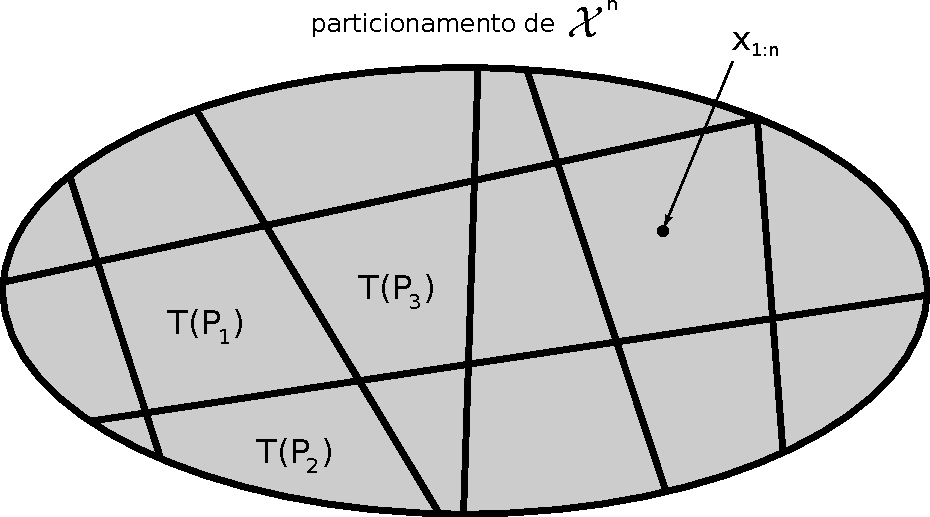
\includegraphics[width=0.8\textwidth]{images/particao-Xn2.pdf}
  %\caption{.}
  \label{fig:particao-Xn}
  \end{figure}
\end{frame}


\subsection{Limite no Número de Tipos}
\begin{frame}[allowframebreaks]
  \frametitle{Limite no Número de Tipos}
  \begin{theorem}[Limite no número de tipos]
  O número de tipos para sequências de comprimento $n$ em um alfabeto $\mathcal{X}$ é limitado por
	\begin{equation}
	\label{eq:number-of-types-bound}
	\vert \mathcal{P}_n \vert \leq (n+1)^{\vert \mathcal{X} \vert} .
	\end{equation}
  \end{theorem}
  \begin{proof}
	\begin{itemize}
	\item Note que o numerador de cada entrada em um tipo pode assumir $(n+1)$ valores distintos (de $0$ a $n$).
	\item Existem $\vert \mathcal{X} \vert$ entradas em um tipo, e portanto a mesma quantidade de numeradores.
	\item Os valores dos numeradores interagem entre si (a soma de todos deve ser igual a $n$), mas podemos
		achar um limite superior desconsiderando esta interação. 
	\item Logo, 
	        \vspace{-2ex}
		\begin{equation}
		\vert \mathcal{P}_n \vert \leq \underbrace{(n+1)\times(n+1)\times\ldots\times(n+1)}_{\vert \mathcal{X} \vert \text{ vezes}} = (n+1)^{\vert \mathcal{X} \vert} .
		\end{equation}
	\end{itemize}
  \end{proof}

  \framebreak
  \begin{itemize}
  \item Importante notar que existe no máximo um número polinomial em $n$ de tipos de sequencias de comprimento $n$.
  \item Além disso, $\exists$ um número exponencial de sequências com comprimento $n$, $\vert \mathcal{X} \vert^n$, e 
	um número (no máximo) polinomial de tipos.
  \item Eventualmente, um dos tipos (um dos blocos na partição) conterá todas as sequências.
  \end{itemize}
\end{frame}
\note{
Note que calcular Equação \ref{eq:number-of-types} é muito mais complicado do que calcular \ref{eq:number-of-types-bound}, e como visto
o limite será suficiente para o que queremos mostrar.
}



\subsection{Probabilidade Depende do Tipo}
\begin{frame}[allowframebreaks]
  \frametitle{Probabilidade Depende do Tipo}
  \begin{theorem}[Probabilidade Depende do Tipo]
	Seja $X_1, X_2, \ldots, X_n$ i.i.d. $\sim Q(x)$, com $Q$ arbitrário, e extensão 
	$Q^n(x_{1:n}) = \prod_i Q(x_i)$, a probabilidade da sequencia depende apenas do tipo, ou seja,
	a probabilidade é `independente' da sequencia, dado o tipo e $Q$, isto é,
	\begin{equation}
	Q^n(x_{1:n}) = 2^{-n[ H(P_{x_{1:n}}) + D(P_{x_{1:n}}||Q) ]}
	\end{equation}
  \end{theorem}
  \begin{itemize}
  \item Probabilidade não depende da sequencia, dado o tipo.
  \item Estatística Suficiente.
  \item Todas as sequencias do mesmo tipo possuem a mesma probabilidade.
  \end{itemize}

  \framebreak
  \begin{proof}
  \vspace{-0.2cm}
  \begin{eqnarray}
  Q^n(x_{1:n}) &=& \prod_{i=1}^{n} Q(x_i) = \prod_{a \in \mathcal{X}} Q(a)^{n(a \mid x_{1:n})} \nonumber \\
	&=& \prod_{a \in \mathcal{X}} Q(a)^{n P_{x_{1:n}}(a) } = \prod_{a \in \mathcal{X}} 2^{ \left\{ n P_{x_{1:n}}(a) \log Q(a) \right\} } \nonumber \\
	&=& \prod_{a \in \mathcal{X}} 2^{ n \left\{  P_{x_{1:n}}(a) \log Q(a) \KeepStyleUnderBrace{ -P_{x_{1:n}}(a) \log P_{x_{1:n}}(a) + P_{x_{1:n}}(a) \log P_{x_{1:n}}(a) }_{=0} \right\} } \nonumber \\
	&=& 2^{n \sum_{a \in \mathcal{X}}  \left( -P_{x_{1:n}}(a) \log \frac{P_{x_{1:n}}(a)}{Q(a)} + P_{x_{1:n}}(a) \log P_{x_{1:n}}(a) \right)  } \nonumber \\
	&=& 2^{-n \left( D(P_{x_{1:n}} \mid \mid Q) + H( P_{x_{1:n}} ) \right) }
  \end{eqnarray}
  \end{proof}

  \framebreak

  \begin{itemize}
  \item (corolário) Se $Q$ é uma distribuição racional (i.e., um tipo possível) e se $x_{1:n} \in T(Q)$, então
	\begin{equation}
	Q^n(x_{1:n}) = 2^{-n H(Q)} .
	\end{equation}
  \item O que ocorre se $Q$ for irracional? Podemos fazer $D(P_{x_{1:n}} \mid \mid Q)$  tão pequeno quando desejável,
	fazendo $n$ grande suficiente.
  \end{itemize}
\end{frame}


\subsection{Tamanho da Classe de Tipo}
\begin{frame}[allowframebreaks]
  \frametitle{Classe de Tipo com maior probabilidade}
  \begin{itemize}
  \item Qual classe de tipo possui maior probabilidade quando a distribuição geradora das sequências é
	$P \in \mathcal{P}_n$?
  \item Considerando a Prop. da Eq. Ass., as sequências típicas são aquelas mais próximas da real distribuição,
	e elas possuem `toda' probabilidade.
  \item Vamos supor então que $T(P)$ possui a maior probabilidade sob a distribuição $P$.
  \end{itemize}

  \begin{lemma}
  Para $P \in \mathcal{P}_n$, teremos que $T(P)$ possui a maior probabilidade. Isto é
	\begin{equation}
	P^n(T(P)) \geq P^n(T(\hat{P})) , \ \forall \hat{P} \in \mathcal{P}_n .
	\end{equation}
  \end{lemma}
  Nota: Sejam $m$ e $n$ inteiros não negativos, então $\frac{m!}{n!} \geq n^{m-n}$. 
	Se $m>n$, então $\frac{m!}{n!} = m(m-1) \ldots (n+1) \geq n^{m-n}$.
	Se $m<n$, então $\frac{m!}{n!} = \frac{1}{n(n-1)\ldots(m+1)} \geq \frac{1}{n^{n-m}}$.
	Se $m=n$, $\frac{m!}{n!} = 1 = n^0$.

  \framebreak

  \begin{proof}
  \vspace{-0.2cm}
  \begin{eqnarray}
  \frac{P^n(T(P))}{P^n(T(\hat{P}))} &=& \frac{\vert T(P) \vert \prod_{a \in \mathcal{X}} P(a)^{nP(a)} }{ \vert T(\hat{P}) \vert \prod_{a \in \mathcal{X}} P(a)^{n\hat{P}(a)}  } \nonumber \\
	&=& \frac{ { n \choose nP(a_1) \ nP(a_2) \ \ldots \ nP(a_D) } \prod_{a \in \mathcal{X}} P(a)^{nP(a)} }{ { n \choose n\hat{P}(a_1) \ n\hat{P}(a_2) \ \ldots \ n\hat{P}(a_D) } \prod_{a \in \mathcal{X}} P(a)^{n\hat{P}(a)}  } \nonumber \\
	&=& \prod_{a \in \mathcal{X}} \frac{ [n\hat{P}(a)]! }{[nP(a)]!} P(a)^{n(P(a)-\hat{P}(a))} \nonumber \\
	&\geq& \prod_{a \in \mathcal{X}} (nP(a))^{n(\hat{P}(a)-P(a))} P(a)^{n(P(a)-\hat{P}(a))} \nonumber \\
	&=& \prod_{a \in \mathcal{X}} n^{n(\hat{P}(a)-P(a))}  
  \end{eqnarray}
  \proofbreak
  \vspace{-2ex}
  \begin{eqnarray}
  \frac{P^n(T(P))}{P^n(T(\hat{P}))} &=& \ldots \nonumber \\
	&\geq& \prod_{a \in \mathcal{X}} n^{n(\hat{P}(a)-P(a))} \nonumber \\
	&=& n^{n\left[ \sum_{a \in \mathcal{X}} \hat{P}(a) - \sum_{a \in \mathcal{X}} P(a) \right]} \nonumber \\
	&=& n^{n(1-1)} = 1
  \end{eqnarray}
  logo, $P^n(T(P)) \geq P^n(T(\hat{P}))$.
  \end{proof}
\end{frame}



\begin{frame}[allowframebreaks]
  \frametitle{Tamanho da Classe de Tipo}
  Podemos expressar o tamanho de uma classe de tipo utilizando os coeficientes multinomiais,
  i.e., o número de maneiras de escolher símbolos distintos do alfabeto para cada elemento
  da sequencia $x_{1:n}$. 

  Para $P \in \mathcal{P}_n$, temos
  \begin{equation}
  \vert T(P) \vert = { n \choose nP(a_1) \ nP(a_2) \ \ldots \ nP(a_n) }
  \end{equation}

  Entretanto, isto é difícil calcular. Queremos encontrar limites que sejam mais facilmente manipulados matematicamente.

  \framebreak

  \begin{theorem}[Limites no tamanho da Classe de Tipo]
  Dado um tipo $P \in \mathcal{P}_n$, temos
	\begin{equation}
	\frac{1}{(n+1)^{\vert \mathcal{X} \vert}} 2^{nH(P)} \leq \vert T(P) \vert \leq 2^{nH(P)}
	\end{equation}
  \end{theorem}
 
  \begin{proof}[limite superior]
  \begin{eqnarray}
  1 &\geq& P^{n} (T(P)) = \sum_{x_{1:n} \in T(P)} P^{n} (x_{1:n}) = \sum_{x_{1:n} \in T(P)} 2^{-nH(P)} \nonumber \\
    &=& \vert T(P) \vert 2^{-nH(P)}
  \end{eqnarray}
  \end{proof}

  \framebreak

  \begin{proof}[limite inferior]
  \begin{eqnarray}
  1 &=& \sum_{Q \in \mathcal{P}_n} P^n (T(Q)) \leq \sum_{Q \in \mathcal{P}_n} \max_{R \in \mathcal{P}_n} P^n (T(R)) \nonumber \\
	 && \text{fazendo } P = \argmax_{R \in \mathcal{P}_n} P^n (T(R)) \text{ teremos } \nonumber \\
	&=& \sum_{Q \in \mathcal{P}_n} P^n (T(P)) \leq (n+1)^{\vert \mathcal{X} \vert} P^n (T(P)) \nonumber \\
	&=& (n+1)^{\vert \mathcal{X} \vert} \sum_{x_{1:n} \in T(P)} P^n (x_{1:n}) \nonumber \\
	&=& (n+1)^{\vert \mathcal{X} \vert} \sum_{x_{1:n} \in T(P)} 2^{-nH(P)} 
  \end{eqnarray} 
  \proofbreak
  \begin{eqnarray}
  1 &=& \ldots \nonumber \\
	&\leq& (n+1)^{\vert \mathcal{X} \vert} \sum_{x_{1:n} \in T(P)} 2^{-nH(P)} \nonumber \\
	&=& (n+1)^{\vert \mathcal{X} \vert} \vert T(P) \vert 2^{-nH(P)}
  \end{eqnarray}
 
  fornecendo assim o resultado
  \begin{equation}
  \vert T(P) \vert \geq \frac{1}{(n+1)^{\vert \mathcal{X} \vert}} 2^{nH(P)}
  \end{equation}
  \end{proof}

\end{frame}

\subsection{Exemplo Binário}
\begin{frame}[allowframebreaks]
  \frametitle{Limites Combinatórios}
  \begin{itemize}
  \item Para o caso binário, $\mathcal{X} = \{0,1\}$, temos os seguintes limites
	\begin{equation}
	\frac{1}{(n+1)^2} 2^{nH(\frac{k}{n})} \leq {n \choose k} \leq 2^{nH(\frac{k}{n})}
	\end{equation}
  \item O limite inferior pode ser ainda mais restrito neste caso 
	\begin{equation}
        \frac{1}{(n+1)} 2^{nH(\frac{k}{n})} \leq {n \choose k} \leq 2^{nH(\frac{k}{n})}
        \end{equation}
  \end{itemize}
\end{frame}

\subsection{Probabilidade da classe de tipo}
\begin{frame}[allowframebreaks]
  \frametitle{Probabilidade da classe de tipo}
   \begin{theorem}
   Para qualquer $P \in \mathcal{P}_n$ e qualquer distribuição $Q$, a probabilidade da classe de tipo
   $T(P)$ sob $Q^n$ é tal que $Q^n(T(P)) \circeq 2^{-n D(P \mid \mid Q)}$. Especificamente, temos os limites
   \begin{equation}
   \frac{1}{(n+1)^{\vert \mathcal{X} \vert}} 2^{-n D(P \mid \mid Q)} \leq Q^n(T(P)) \leq 2^{-nD(P \mid \mid Q)}
   \end{equation}
   \end{theorem}
   obs.: qualquer tipo menos próximo do tipo mais próximo de $Q$ irá ter probabilidade exponencialmente decrescente com $n$, 
   decrescendo mais rapidamente que o tipo mais provável.
   \framebreak
   \begin{proof}
   \begin{eqnarray}
   Q^n(T(P)) &=& \sum_{x_{1:n} \in T(P)} Q^n(x_{1:n}) = \sum_{x_{1:n} \in T(P)} 2^{-n (D(P \mid \mid Q) + H(P))} \nonumber \\
	&=& \vert T(P) \vert 2^{-n (D(P \mid \mid Q) + H(P))}
   \end{eqnarray}
   para completar a demonstração, devemos utilizar 
        \begin{equation}
        \frac{1}{(n+1)^{\vert \mathcal{X} \vert}} 2^{nH(P)} \leq \vert T(P) \vert \leq 2^{nH(P)}
        \end{equation}
   \end{proof}

   \framebreak

   \begin{itemize}
   \item Quais tipos terão maior probabilidade?
   \item Claramente aqueles mais próximos da real distribuição.
   \item A propriedade $Q^n(T(P)) \circeq 2^{-n D(P \mid \mid Q)}$ diz que aqueles
	mais distantes terão probabilidade exponencialmente menor do que os demais, quando $n \rightarrow \infty$.
   \end{itemize}

\end{frame}


\subsection{Sumário}
\begin{frame}[allowframebreaks]
  \frametitle{Sumário}
   \begin{itemize}
   \item Número de tipos de sequências com comprimento $n$
	\begin{equation}
	\vert \mathcal{P}_n \vert \leq (n+1)^{\vert \mathcal{X} \vert}
	\end{equation}
   \item A probabilidade da sequência ($p(x_{1:n})$) depende apenas do tipo 
	\begin{equation}
	Q^n(x_{1:n}) = 2^{-n [H(P_{x_{1:n}}) + D(P_{x_{1:n}} \mid \mid Q)]}
	\end{equation}
   \item Tamanho da Classe de Tipo
	\begin{equation}
	\vert T(P) \vert \circeq 2^{nH(P)}
        \end{equation}
   \item Probabilidade da classe de tipo
	\begin{equation}
	Q^n(T(P)) \circeq 2^{-nD(P \mid\mid Q)}
	\end{equation}
   \end{itemize}
\end{frame}



\subsection{Conjunto Típico}
\begin{frame}[allowframebreaks]
  \frametitle{Conjunto Típico}
  \begin{itemize}
  \item Os tipos $P$ mais próximos da real distribuição $Q$ terão maior probabilidade.
  \item Aqueles mais distantes de $Q$ terão probabilidade exponencialmente menor do que os demais.
  \end{itemize}

   \begin{definition}[conjunto típico de sequências]
   Seja $X_1, X_2, \ldots, X_n$ i.i.d. $\forall i$, $X_i \sim Q(x)$. Então o conjunto típico é definido como
        \begin{equation}
        T^{\epsilon}_{Q} = \{ x_{1:n} : D(P_{x_{1:n}} \mid \mid Q) \leq \epsilon \}
        \end{equation}
   \end{definition}

   \framebreak

  \begin{theorem}[probabilidade do conjunto típico]
  Sejam $X_1, X_2, \ldots, X_n$ i.i.d. $\forall i$, $X_i \sim Q(x)$. A probabilidade do complemento
  do conjunto típico $\overline{T}^{\epsilon}_Q$ é dada por
	\begin{equation}
	Q(\overline{T}^{\epsilon}_Q) = Q( \{ x_{1:n} : D(P_{x_{1:n}} \mid\mid Q) > \epsilon  \} ) \leq 2^{-n (\epsilon - \vert \mathcal{X} \vert \frac{\log (n+1)}{n})}
	\end{equation}
  desta forma
	\begin{equation}
	D(P_{x_{1:n}} \mid\mid Q) \xrightarrow{p} 0 \text{ quando } n \rightarrow \infty
	\end{equation}
  (converge em probabilidade para zero quando $n$ é grande suficiente)
  \end{theorem}
  \begin{itemize}
  \item Os tipos que divergem (KL) mais do que $\epsilon$ da distribuição subjacente $Q$ terão probabilidade decrescente. 
  \item Para $n$ grande, o conjunto típico acaba sendo a única coisa que ocorre com uma probabilidade não evanescente.
  \end{itemize} 

  \framebreak

  \begin{proof}
  \begin{eqnarray}
  1 - Q^{n}(T^{\epsilon}_Q) &=& Q(\overline{T}^{\epsilon}_Q) = \sum_{P \in \mathcal{P}_n : D(P \mid\mid Q) > \epsilon} Q^n (T(P)) \nonumber \\
	&\leq& \sum_{P \in \mathcal{P}_n : D(P \mid\mid Q) > \epsilon} 2^{-n D(P\mid\mid Q)} \nonumber \\
	&\leq& \sum_{P \in \mathcal{P}_n : D(P \mid\mid Q) > \epsilon} 2^{-n \epsilon} \nonumber \\
	&\leq& (n+1)^{\vert \mathcal{X}  \vert} 2^{-n \epsilon} = 2^{-n \left( \epsilon - \vert \mathcal{X} \vert \frac{\log (n+1)}{n}  \right)}
  \end{eqnarray}
  então a probabilidade vai para zero quando $n \rightarrow \infty$, e desta forma a probabilidade do conjunto típico vai para $1$ quando $n \rightarrow \infty$.
  \end{proof}

  \framebreak

  \begin{itemize}
  \item Com qual frequência um evento atípico ocorre?
  \item Como $p(\overline{T}^{\epsilon}_Q) \leq 2^{-n \left( \epsilon - \vert \mathcal{X} \vert \frac{\log (n+1)}{n}  \right)}$, uma 
	sequencia em $n$ exponencial decrescente. Esta será, desta forma, somável.
	\begin{equation}
	\infty > \sum_{n=1}^{\infty} p(D(P_{x_{1:n}} \mid\mid Q) > \epsilon) = E_Q \left[ \sum_{n=1}^{\infty} \mathbf{1}_{\{ D(P_{X_{1:n}} \mid\mid Q) > \epsilon \}}  \right]
	\end{equation}
  \item O número esperado de vezes que o evento $D(P_{X_{1:n}} \mid\mid Q) > \epsilon$ ocorre é finito, dentro de um conjunto infinito de possíveis ocorrências.
  \end{itemize}
\end{frame}




\subsection{Codificação Universal de Fonte}
\begin{frame}[allowframebreaks]
  \frametitle{Codificação Universal de Fonte}
  \begin{itemize}
  \item Dizemos que uma codificação de fonte é universal quando ela não depende de $p(x)$.
  \item Codificação não universal: Se conhecemos $p(x)$, podemos propor um código para comprimir a fonte caracterizada por $p(x)$.
	Exemplo: Código de Huffman.
  \item É possível criar um código universal (não dependente de $p(x)$) que atinja o limite da entropia? taxa $R > H(Q)$ (em bits por símbolo)
  \item O que ocorre se $R < H(Q)$?
  \item Ideia similar àquela do conjunto típico $A_{\epsilon}^{(n)}$. Vamos codificar apenas aquilo que de fato ocorre.
	Precisaremos de no máximo $\vert A_{\epsilon}^{(n)} \vert$ palavras que podem ser indexadas com $nH$ bits.
  \item Vamos formalizar o teorema de Shannon utilizando o método de tipo.
  \end{itemize}

  \framebreak

  \begin{itemize}
  \item Existem no máximo $2^{nH(P)}$ sequências do tipo $P$. Podermos utilizar $nH(P)$ bits para representar tais sequencias.
  \item Se $R > H(P)$, podemos utilizar $nR$ bits para representar estas sequências.
  \item Quando $n$ cresce, apenas os tipos $P$ `próximos' de $Q$ irão ocorrer.
  \item Existe um número exponencial (em $n$) de sequências e um número polinomial (em $n$) de tipos.
  \item Eventualmente, um tipo terá `toda' a probabilidade.
  \end{itemize}

  \framebreak
 
  \begin{figure}[h!]
  \centering
  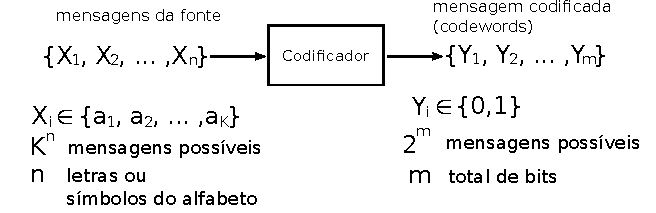
\includegraphics[width=0.9\textwidth]{images/blockcoding.pdf}
  %\caption{.}
  \label{fig:blockcoding-types}
  \end{figure}

\end{frame}


\begin{frame}[allowframebreaks]
  \frametitle{Códigos $(M,n)$}
  \begin{itemize}
  \item código de blocos com taxa fixa $R$
  \item Existem $M$ palavras. $M$ é o número de possíveis mensagens.
  \item $n$ símbolos são codificados conjuntamente a cada instante.
  \item O codificador faz o mapeamento de \textit{strings} de tamanho $n$ produzidas pela fonte em \textit{strings} de $m$ bits.
    \begin{figure}[h!]
    \centering
    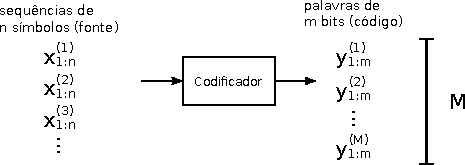
\includegraphics[width=0.9\textwidth]{images/Mncodes2.pdf}
    %\caption{.}
    \label{fig:Mncodes}
    \end{figure}
  \item A taxa $R$ depende de $M$ e $n$.
	\begin{equation}
	R = \frac{\log M}{n} = \frac{\log (\text{n. de palavras}) }{\text{n. de símbols}}
	\end{equation}
  \end{itemize}

  \framebreak

  \begin{definition}[código de bloco com taxa fixa $R$]
  Seja $X_1, X_2, \ldots, X_n \sim Q$, i.i.d. mas $Q$ desconhecido. A função do codificador
  e decodificador são definidas a seguir:
	\begin{equation}
	\text{codificador: } f_n : \mathcal{X}^n \rightarrow \{1,2,\ldots,2^{nR}\}
	\end{equation}
	\begin{equation}
        \text{decodificador: } \phi_n : \{1,2,\ldots,2^{nR}\} \rightarrow \mathcal{X}^n
	\end{equation}
  e a probabilidade de erro
	\begin{equation}
	P_e^{(n)} = Q^n (\{ x_{1:n} : \phi (f_n (x_{1:n})) \neq x_{1:n} \})
        \end{equation}	
  \end{definition}

  \framebreak

  \begin{definition}[código de bloco universal de taxa $R$]
  Um código de bloco de taxa $R$ para um fonte é dito universal se a função $f_n$ e $\phi_n$
  não depender da distribuição $Q$ e se 
	\begin{equation}
	P_e^{(n)} \rightarrow 0 \text{ quando } n \rightarrow \infty \text{ sempre que } H(Q) < R
        \end{equation}
  \end{definition}
  \begin{itemize} 
  \item Se $R > H(Q)$, então existe uma sequência (em $n$) de códigos com erro evanescente.
  \item Por outro lado, se $R < H(Q)$ a probabilidade de erro vai pra 1.
  \end{itemize}
\end{frame}


\subsection{Teorema da Codificação de Shannon}

\begin{frame}[allowframebreaks]
  \frametitle{Simplex Probabilístico}

  \begin{definition}[Simplex Probabilístico]
  O Simplex Probabilístico em $\RealNumber^m$ é o conjunto de pontos
  $x_{1:m} = (x_1, x_2, \ldots, x_m) \in \RealNumber^m$ tal que $x_i \geq 0$, $\sum_{i=1}^{m} x_i = 1$.
  \end{definition}
  \framebreak 
  \begin{example}[$m=2$]
  O Simplex probabilístico será o conjunto de pontos
  \begin{equation}
  \{ (x_1, x_2)  :  x_1 \geq 0 , x_2 \geq 0 , x_1 + x_2 = 1 \}
  \end{equation}
    \begin{figure}[h!]
    \centering
    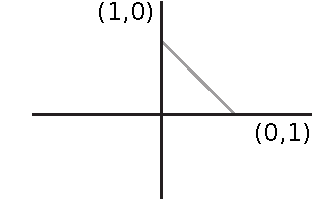
\includegraphics[width=0.4\textwidth]{images/prob-simplex-2.pdf}
    %\caption{.}
    \label{fig:prob-simplex-2}
    \end{figure}

  \end{example}
  \framebreak
  \begin{example}[$m=3$]
  O Simplex probabilístico será o conjunto de pontos
  \begin{equation}
  \{ (x_1, x_2, x_3)  :  x_1 \geq 0 , x_2 \geq 0 , x_3 \geq 0 , x_1 + x_2 + x_3 = 1 \}
  \end{equation}

    \begin{figure}[h!]
    \centering
    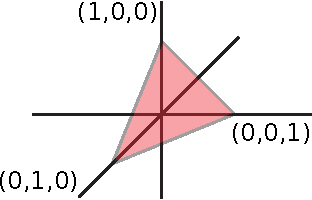
\includegraphics[width=0.4\textwidth]{images/prob-simplex-3.pdf}
    %\caption{.}
    \label{fig:prob-simplex-3}
    \end{figure}

  \end{example}

  \framebreak
  Os tipos em para $\vert \mathcal{X} \vert = m$ podem ser representados em um Simplex Probabilístico em $\RealNumber^m$.
  \begin{example}[$\vert \mathcal{X} \vert = 3$]
    \begin{figure}[h!]
    \centering
    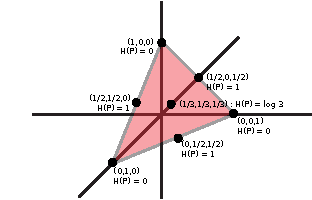
\includegraphics[width=0.5\textwidth]{images/prob-simplex-types3.pdf}
    %\caption{.}
    \label{fig:prob-simplex-3}
    \end{figure}
  \end{example}

\end{frame}


\begin{frame}[allowframebreaks]
  \frametitle{Teorema da Codificação de Shannon}
  \begin{theorem}[Teorema da Codificação de Shannon]
  $\exists$ uma sequencia $(2^{nR},n)$ de códigos universais tais que $P_e^{(n)} \rightarrow 0$ para toda
  distribuição $Q$ tal que $H(Q) < R$.
  \end{theorem}

  \framebreak 

  \begin{proof}
  \begin{itemize}
  \item Fixe $R > H(Q)$.
  \item Defina uma taxa para $n$ que é fixada a um fator polinomial.
	\begin{equation}
	R_n \triangleq R - \vert \mathcal{X} \vert \frac{\log (n+1)}{n} < R
	\end{equation}
  \item Defina um conjunto de sequências que possuem entropia de tipo menor do que esta taxa.
	\begin{eqnarray}
	A_n &\triangleq& \{ x_{1:n} \in \mathcal{X}^n : H(P_{x_{1:n}}) \leq R_n \} \nonumber \\
		&=& \left\{  \bigcup_{P \in \mathcal{P}_n} T(P) : H(P) \leq R_n \right\}
	\end{eqnarray}
  \end{itemize}
 
  \proofbreak

  \begin{itemize}
  \item Temos então
  \begin{eqnarray}
	\vert A_n \vert &=& \sum_{P \in \mathcal{P}_n : H(P) \leq R_n} \vert T(P) \vert \leq \sum_{P \in \mathcal{P}_n : H(P) \leq R_n} 2^{nH(P)} \nonumber \\
			&\leq& \sum_{P \in \mathcal{P}_n : H(P) \leq R_n} 2^{nR_n} \leq (n+1)^{\vert \mathcal{X} \vert} 2^{nR_n} \nonumber \\
			&=& 2^{n \left( R_n + \vert \mathcal{X} \vert \frac{\log (n+1)}{n} \right)} = 2^{nR} .
  \end{eqnarray}
  \item Como $\vert A_n \vert \leq 2^{nR}$, podemos indexar $A_n$ com $nR$ bits.
  \end{itemize}  

  \proofbreak

  O codificador será dada por
  \begin{equation}
  f_n (x_{1:n}) = \begin{cases} 
		\text{índice de } x_{1:n} \text{ em } A_n ,	\quad \text{ se } x_{1:n} \in A_n \\
		0					,	\quad \text{ caso contrário }.
		\end{cases}
  \end{equation}

  \begin{itemize}
  \item O codificador associará um índice a $x_{1:n}$ se $H(P_{x_{1:n}}) \leq  R_n$ (ou seja, $x_{1:n} \in A_n$); 
  e não associará valor se $H(P_{x_{1:n}}) >  R_n$ (ou seja, $x_{1:n} \notin A_n$).
  \item Note que $f_n(\cdot)$ não depende da distribuição da fonte, apenas do ordenamento e de $\RealNumber^m$.
  \item Um erro ocorrerá se $x_{1:n} \notin A_n$.
  \end{itemize}
  
  \proofbreak
  Os tipos podem ser representados por pontos em um Simplex Probabilístico.
    \begin{figure}[h!]
    \centering
    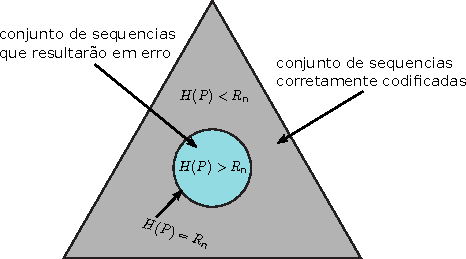
\includegraphics[width=0.5\textwidth]{images/type-simplex.pdf}
    %\caption{.}
    \label{fig:type-simplex}
    \end{figure}

  \proofbreak

  Um erro ocorre quando a sequência não está em $A_n$. Desta forma,
  \begin{eqnarray}
  P_e^{(n)} &=& 1 - Q^n(A_n) = \sum_{P: H(P) > R_n} Q^n (T(P)) \nonumber \\
	&\leq& \sum_{P: H(P) > R_n} \max_{P: H(P) > R_n} Q^n (T(P)) \nonumber \\
	&\leq& (n+1)^{\vert \mathcal{X} \vert} \max_{P: H(P) > R_n} Q^n (T(P)) \nonumber \\
	&\leq& (n+1)^{\vert \mathcal{X} \vert} \max_{P: H(P) > R_n} 2^{-n  D(P \mid\mid Q)} \nonumber \\
	&=& (n+1)^{\vert \mathcal{X} \vert} 2^{-n [\min_{P: H(P) > R_n} D(P \mid\mid Q)]}
  \end{eqnarray}
  %onde utilizamos que $Q^n(T(P)) \leq 2^{-n D(P\mid \mid Q)}$.


  \proofbreak

  \begin{itemize}
  \item Temos que $R_n$ forma uma sequência crescente com $n$, tal que $R_n < R$ para todo $n$.
  \item Por hipótese, $H(Q) < R$.
  \item Eventualmente, para algum $n_0$, teremos que $\forall n > n_0$, $R_n > H(Q)$.
  \item Na equação anterior, escolhemos $P: H(P) > R_n$.

    \begin{figure}[h!]
    \centering
    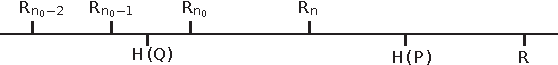
\includegraphics[width=0.9\textwidth]{images/Rn-seq.pdf}
    %\caption{.}
    \label{fig:Rn-seq}
    \end{figure}

  \item Teremos então: $H(P) > R_n > H(Q)$, o que implica em $P \neq Q$.
  \item Desta forma, teremos $D(P \mid\mid Q) > 0$ para $P$ escolhido.
  \end{itemize}


  \proofbreak

  \begin{itemize}
  \item Teremos assim
	\begin{equation}
	P_e^{(n)} \leq \underbrace{(n+1)^{\vert \mathcal{X} \vert}}_{\text{polinomial em } n} \underbrace{ 2^{-n [\min_{P: H(P) > R_n} D(P \mid\mid Q)]} }_{\text{exp. decrescente qnd } n \rightarrow \infty}
	\end{equation}
  \item Logo, $P_e^{(n)} \rightarrow 0$ quando $n \rightarrow \infty$.
  \end{itemize}


  \end{proof}

  \begin{itemize}
  \item Por outro lado, se $R < H(Q)$ teremos $P_e^{(n)} \rightarrow 1$.
  \item Entropia é o limite de compressão.
  \end{itemize}

\end{frame}


